\documentclass[a4paper,UKenglish,cleveref, autoref, thm-restate]{lipics-v2021}
\usepackage{xspace}
\usepackage{graphicx} % For \includegraphics
%\graphicspath{{./graphics/}}%helpful if your graphic files are in another directory
\usepackage{amsmath}
\bibliographystyle{plainurl}% the bibstyle
\usepackage{cleveref} % Provides \Cref
\usepackage{listings} % For code snippets


\title{Implementation and verification of encoder, decoder and generator for prefix-free codes}

\author{Samuel Chassot}{EPFL}{samuel.chassot@epfl.ch}{}{}
\author{Daniel Filipe Nunes Silva}{EPFL}{daniel.nunessilva@epfl.ch}{}{}

\authorrunning{S.~Chassot and D.~F.~Nunes~Silva}

\Copyright{Samuel Chassot and Daniel Filipe Nunes Silva}

\ccsdesc[500]{Software and its engineering~Software verification and validation}

\keywords{formal verification, prefix-free codes, Huffman Coding}

\category{}
\relatedversion{}
\supplement{}
\nolinenumbers 
\hideLIPIcs

\begin{document}

\maketitle

\begin{abstract}
    We propose an implementation in the Scala programming language of an encoder, a decoder as well as a naive prefix-free code generator. These implementations are formally proven for correctness thanks to the verification framework Stainless \cite{stainless}. Those three functions can be chained to form a pipeline as a whole on a given input string $s$, i.e. generate a correspoding prefix-free code $c$, use $c$ to encode $s$ as $e$ and finally decode $e$ with $c$ as $d$. Correctness is therefore defined as $s == d$.
\end{abstract}

\definecolor{bgcolor}{RGB}{240,252,210}
\definecolor{kwcolor}{RGB}{0,0,200}
\lstdefinelanguage{scala}{
  keywordstyle=\color{kwcolor},
  backgroundcolor=\color{bgcolor},
  alsoletter={@,=,>},
  morekeywords={abstract, case, class, def,
        else, extends, false, free, if, implicit, match,
        object, true, val, var, while, sealed,
        for, dependent, null, type, with, try, catch, finally,
        import, final, return, new, override, this, trait,
        private, public, protected, package, throw},
  sensitive=true,
  morecomment=[l]{//},
  morecomment=[s]{/*}{*/},
  morestring=[b]",
  mathescape=true,
  %emph={Int,Char,Boolean,String,Unit},
  %emphstyle={\color{blue}}
}
\lstset{language=scala}


\section{Introduction}
\label{sec:intro}

The aim of this project is to come up with a verified implementation of an encoder and decoder pair as well as a prefix-free code generator in the scope of a personal project for the Formal Verification course (CS-550) at EPFL.

In \cite{blanchette}, J. C. Blanchette presents a formal proof of the optimality for the Huffman's algorithm. The latter generates a prefix-free code for a string such that the encoding of the encoded string has minimal length. As proposed in the conclusion of Blanchette's article, we explore the verification of encode/decode functions.

In this report, we start with some background knowledge related to prefix-free codes. Then, we go through the verified implementation of the pipeline we propose.

\subsection*{Prior work}

To the best of our knowledge, this is the first time an encode/decode function pair is formally verified.
However we can find many examples of similar exercises in the litterature such as a formal definition Huffman's algorithm in \cite{formal} or a formally verified implemention of compression/decompression function pair for deflate in \cite{deflate}.

\subsection*{Our approach} % the star makes the section number disappear

We first consider the whole class of prefix-free codes and not only the optimal ones generates by Huffman's algorithm.
Then, we come up with basic datatypes and implementations plain Scala code before adding  \emph{require}s and \emph{ensuring}s from Stainless in order to validate the main correctness theorem.
Finally, we also implement and verify an naive prefix-free code generator in order to complete the whole pipeline.

\subsection*{Contributions} % the star makes the section number disappear

The main contributions of this report are the following:
\begin{enumerate}
    \item a formally verified implementation of an encode function for prefix-free codes
    \item a formally verified implementation of an decode function for prefix-free codes
    \item a formally verified implementation of a prefix-free code generator
\end{enumerate}

\section{Implementation}

Our code is available in the following repository:
\begin{center}
    \url{https://github.com/samuelchassot/FormalVerification-Project}
\end{center}
and build instructions are in file \verb|README.md| in the top-level directory.

\section{Prefix-free codes} %TODO

We define a code as a map from a list of characters formed from a string, the symbols, to a list of bits, the code words. The fact that a code is prefix-free means that there is no full code word in this map that is a prefix of an other code word, i.e. $01$ is a prefix of the code word $0111$.

Those codes can be represented as full binary trees. To determine the code word of a symbols located in the leaves, it suffices to find the path from the root down to the corresponding leaf assuming that taking the left child represents the 0 bit and the right child represents the 1 bit.

{'a': 0, 'b': 10, 'c': 110, 'd': 111} is a prefix-free code and the correponding full binary tree can be seen in figure~\ref{fig:pfc}.
\begin{figure}[ht]
    \centering
    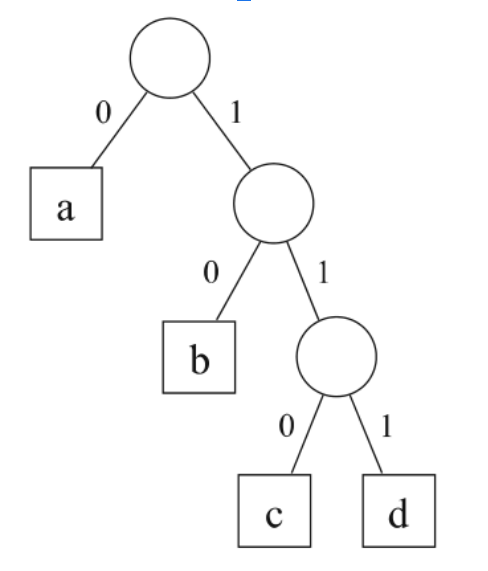
\includegraphics[width=0.3\textwidth]{pfc.png}
    \caption{A full binary tree representing a prefix-free code.\label{fig:pfc}}
\end{figure}

\section{Datatypes} %TODO

We represent a string (the tyoe of an input of the pipeline) as \lstinline{List[Char]} as it is easier to define recursion using lists rather than the \lstinline{String} type directly. 
Similarily we define an encoded binary string (the type of an output of the pipeline) as \lstinline{List[Boolean]}.

To represent the binary trees used to represent the prefix-free codes, we define the folowing case classes:

\begin{lstlisting}
    sealed abstract class Tree
    case class InnerNode(t1: Tree, t2: Tree) extends Tree
    case class Leaf(w: BigInt, c: Char) extends Tree
  
    type Forest = List[Tree]
\end{lstlisting}

A \lstinline{Forest} is a list of trees that is used in the process of generation of the prefix-free code.

\section{Encode} %TODO

TODO

\section{Decode} %TODO

TODO

\section{Prefix-free code generator} %TODO

TODO

\section{Future work} %TODO

Huffman's algorithm was the starting point of this project altough we did not clearly exploit it. We restricted ourselves to the broader class of prefix-free codes and how to generate some without worrying about its optimality as in \cite{blanchette}. 

As an improvement, we suggest to extend our current implementation of naive prefix-free code generator to an actual formally verified implementation of Huffman's algorithm. This is surely more challenging to prove since Huffman's algorithm requires sorting the forest of tree at each iteration. Ensuring the forest properties such as the characters that can be uniquely decoded with it, is not trivial.

\section{Conclusions} %TODO

TODO

\vspace{0.5cm} % somem vertical space since we are creating this paragraph manually
\noindent % otherwise many styles like to indent the first word of a paragraph
\textbf{\large Acknowledgements.}\ % Bold, large font
The autors of this report would like to thank Viktor Kun\v{c}ak for proposing such course at EPFL and offering to get some experience with a personal project they truly enjoyed to work on. The autors thank Jad Hamza, who was often able to provide precious help for the progress of the project despite the lack of context.

% =======================================================================================

\bibliography{main} % this will make bibliography appear

\end{document}
